\documentclass[a4paper,11pt]{article}

% --- Paketit ---
\usepackage[utf8]{inputenc}
\usepackage[T1]{fontenc}
\usepackage[finnish]{babel}
\usepackage{amsmath, amssymb, amsthm}
\usepackage{geometry}
\geometry{left=3cm, right=3cm, top=3cm, bottom=3cm}

% --- Grafiikka ja kuvaajat (TikZ & PGFPlots) ---
\usepackage{tikz}
\usetikzlibrary{positioning, automata, arrows.meta}
\usepackage{pgfplots}
\pgfplotsset{compat=1.18}
\usepgfplotslibrary{fillbetween}


% --- Laatikko ---
\usepackage[most]{tcolorbox}

\newtcolorbox{derivationbox}[1][]{
  breakable,                % Sallii laatikon jakautumisen sivunvaihdossa
  enhanced,
  colback=gray!5,          % Hyvin vaalea harmaa tausta
  colframe=gray!50!black,  % Tummanharmaa reunus
  title={#1},              % Otsikko parametrista
  fonttitle=\bfseries\sffamily,
  attach boxed title to top left={yshift=-2mm, xshift=2mm},
  boxed title style={
    colback=gray!50!black,
    sharp corners
  },
  %sharp corners=south,     % Alakulmat terävät
  arc=3mm,                 % Yläkulmat pyöristetyt
  parbox=false             % Sallii tavallisen tekstin ja kaavat
}

% --- Tyyliasetukset ---
\setlength{\parindent}{0pt}
\setlength{\parskip}{1em}
\linespread{1.1}

% --- Otsikointi ---
\title{Optimointimallin matemaattinen johto}
\author{Elias Ervamaa}
\date{\today}

\begin{document}

\maketitle

\section{Johdanto}
Tässä dokumentissa johdetaan analyyttinen ratkaisu kahden jonon resurssien allokointiongelmalle. Tarkastelu etenee kahdessa vaiheessa: ensin johdetaan yksittäisen M/M/1-jonon odotusajan lauseke, minkä jälkeen ratkaistaan optimointiongelma Lagrangen kertoimien menetelmällä.

\subsection{Muuttujat}
Mallissa käytetään seuraavia merkintöjä:
\begin{itemize}
    \item $\lambda_i \in \mathbb{N}$: Saapumisintensiteetti (asiakasta / aikayksikkö).
    \item $\mu_i \in \mathbb{R}_+$: Palvelunopeus (palvelua / aika / työntekijä).
    \item $x_i \in \mathbb{R}_+$: Työntekijöiden määrä.
    \item $w_i \in \mathbb{R}_+$: Odotusajan painokerroin ("haittakerroin").
    \item $c_i \in \mathbb{R}_+$: Työntekijän yksikkökustannus.
    \item $B \in \mathbb{R}_+$: Kokonaisbudjetti.
\end{itemize}

\newpage
\section{Todennäköisyysjakaumat}

\subsubsection*{Saapumisprosessi (Poisson)}
Asiakkaiden saapuminen noudattaa Poisson-prosessia. Todennäköisyys sille, että aikayksikössä ($t$) saapuu tasan $k$ asiakasta, on:
\begin{equation}
    P(X=k) = \frac{\lambda^k e^{-\lambda}}{k!}, \quad k = 0, 1, 2, \dots
\end{equation}

\begin{center}
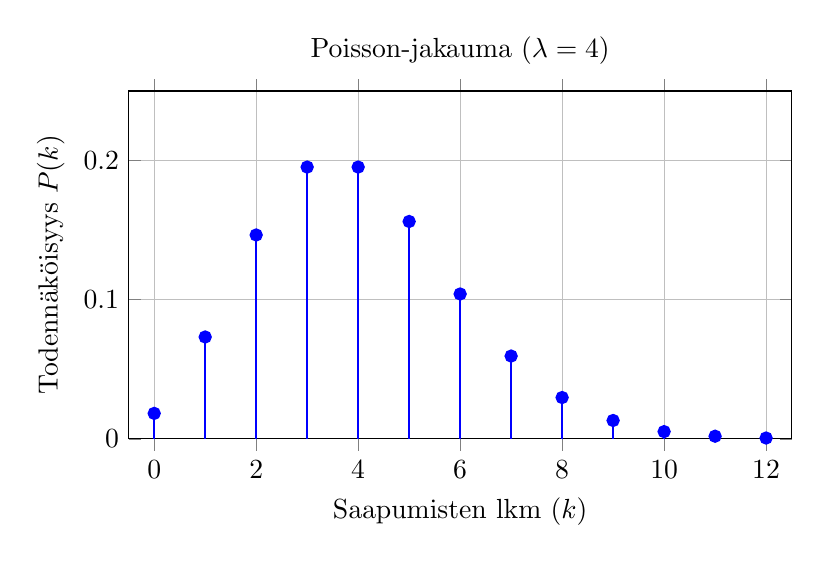
\begin{tikzpicture}
\begin{axis}[
    width=10cm, height=6cm,
    title={Poisson-jakauma ($\lambda=4$)},
    xlabel={Saapumisten lkm ($k$)},
    ylabel={Todennäköisyys $P(k)$},
    ymin=0, ymax=0.25,
    xmin=-0.5, xmax=12.5,
    ybar,
    bar width=2pt,
    grid=major
]
    \addplot+[ycomb, blue, thick, mark=*] coordinates {
        (0, 0.0183) (1, 0.0732) (2, 0.1465) (3, 0.1953) (4, 0.1953)
        (5, 0.1562) (6, 0.1041) (7, 0.0595) (8, 0.0297) (9, 0.0132)
        (10, 0.0052) (11, 0.0019) (12, 0.0006)
    };
\end{axis}
\end{tikzpicture}
\end{center}

\subsubsection*{Palveluajat (Eksponentti)}
Palveluajat $T$ noudattavat eksponenttijakaumaa. Tiheysfunktio on:
\begin{equation}
    f(t; \mu) = \mu e^{-\mu t}, \quad t \ge 0
\end{equation}
Tässä $\mu$ kuvaa palvelunopeutta (rate), joten keskimääräinen palveluaika on $E[T] = 1/\mu$.

\begin{center}
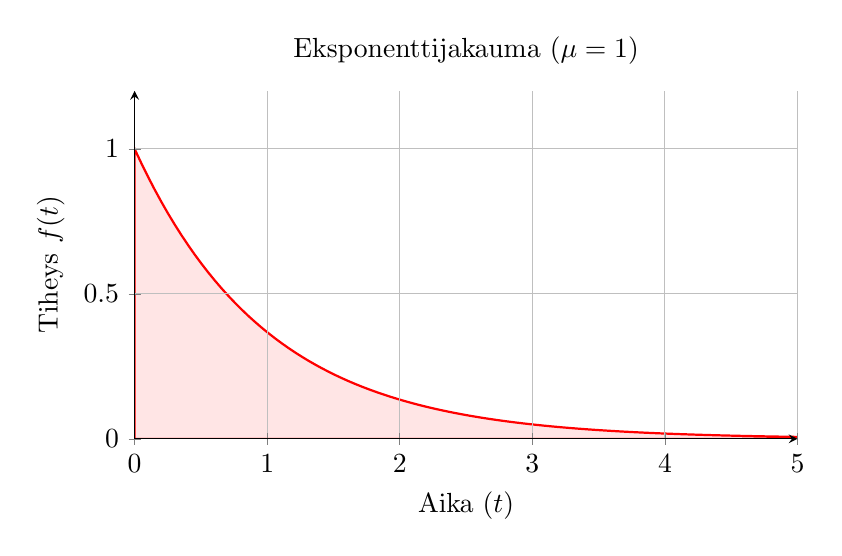
\begin{tikzpicture}
\begin{axis}[
    width=10cm, height=6cm,
    title={Eksponenttijakauma ($\mu=1$)},
    xlabel={Aika ($t$)},
    ylabel={Tiheys $f(t)$},
    domain=0:5, samples=100,
    ymin=0, ymax=1.2,
    axis lines=left,
    grid=major,
    axis on top
]
    \addplot [thick, red, fill=red!10] {exp(-x)} \closedcycle;
\end{axis}
\end{tikzpicture}
\end{center}

\newpage


\section{M/M/1-jonon johtaminen}
\subsection{Tasapainoehto}

% Jotta jono pysyisi tasapainotilassa eikä kasvaisi rajatta, on $x > \frac{\lambda}{\mu}$ (eli $\rho < 1$). Oletetaan, että on kulunut tietty aika, jonka jälkeen jonon jakauma on vakaassa tilassa:

Mallinnetaan yhtä jonoa jatkuva-aikaisena Markov-ketjuna. Systeemin tila $n \in \{0, 1, 2, \dots\}$ kertoo asiakkaiden kokonaismäärän (jonossa + palvelussa).
Systeemin dynamiikka perustuu kahteen voimaan:
\begin{itemize}
    \item \textbf{Saapuminen:} Uusi asiakas saapuu intensiteetillä $\lambda$, mikä nostaa tilaa ($n \to n+1$).
    \item \textbf{Poistuminen:} Palvelu valmistuu intensiteetillä $x\mu$, mikä laskee tilaa ($n \to n-1$). Tämä on mahdollista vain, kun systeemissä on asiakkaita ($n \ge 1$).
\end{itemize}

Määritellään liikennekuorma $\rho = \frac{\lambda}{x\mu}$.
Systeemin stabiilisuus vaatii ehdon $x > \frac{\lambda}{\mu}$ (eli $\rho < 1$).
Oletetaan, että systeemi on ollut toiminnassa riittävän kauan, jolloin alkutilanteen vaikutus on hävinnyt ja systeemi on saavuttanut stokastisen tasapainon. Tämä tapahtuu koska $\rho < 1$, jono ei kasva äärettömyyksiin, vaan todennäköisyysjakauma $p_n$ stabiloituu ajasta riippumattomaksi vakiojakaumaksi. Tässä vakaassa tilassa todennäköisyysvirta tilojen välillä tasaantuu: pitkällä aikavälillä keskimääräinen siirtymä mihin tahansa tilaan $n$ täytyy olla yhtä suuri kuin siirtymä sieltä pois.

Voimme visualisoida tämän tilakaaviona, jossa ympyrät kuvaavat tiloja ja nuolet siirtymäintensiteettejä:



\begin{center}
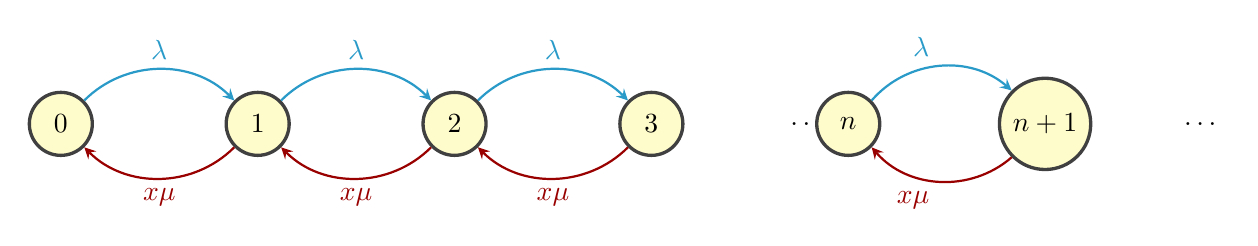
\begin{tikzpicture}[>=stealth, node distance=2.5cm, on grid, auto, initial text=, initial where=left]
    % Tyylit
    \tikzstyle{state}=[circle, draw=black!75, fill=yellow!20, very thick, minimum size=8mm]
    \tikzstyle{arrow}=[->, thick, draw=blue!50!black]

    % Tilat (Solmut)
    \node[state] (0) {0};
    \node[state] (1) [right=of 0] {1};
    \node[state] (2) [right=of 1] {2};
    \node[state] (3) [right=of 2] {3};
    \node (4) [right=of 3, xshift=-0.5cm] {$\dots$}; % Pisteet
    \node[state] (k) [right=of 3] {$n$};
    \node[state] (k1) [right=of k] {$n+1$};
    \node (end) [right=of k1, xshift=-0.5cm] {$\dots$};

    % Siirtymät (Nuolet)
    % Lambda (oikealle)
    \draw[arrow, cyan!80!black] (0) edge [bend left=45] node {$\lambda$} (1);
    \draw[arrow, cyan!80!black] (1) edge [bend left=45] node {$\lambda$} (2);
    \draw[arrow, cyan!80!black] (2) edge [bend left=45] node {$\lambda$} (3);
    \draw[arrow, cyan!80!black] (k) edge [bend left=45] node {$\lambda$} (k1);

    % Mu (vasemmalle) - Huom: mallissa teho on x*mu
    \draw[arrow, red!60!black] (1) edge [bend left=45] node {$x\mu$} (0);
    \draw[arrow, red!60!black] (2) edge [bend left=45] node {$x\mu$} (1);
    \draw[arrow, red!60!black] (3) edge [bend left=45] node {$x\mu$} (2);
    \draw[arrow, red!60!black] (k1) edge [bend left=45] node {$x\mu$} (k);

\end{tikzpicture}
\end{center}

Tarkastellaan leikkausta kahden tilan välissä. Jotta tilannetta kuvaava todennäköisyysjakauma $p_n$ pysyisi vakiona, täytyy virran leikkauksen yli oikealle olla yhtä suuri kuin virran vasemmalle.
Tästä saamme \textbf{globaalin tasapainoyhtälön}:

\begin{equation*}
    \underbrace{\lambda \cdot p_n}_{\text{Virta ylös } (n \to n+1)} = \underbrace{x\mu \cdot p_{n+1}}_{\text{Virta alas } (n+1 \to n)}
\end{equation*}

\textbf{Erikoistapaus}
Systeemi siirtyy tyhjästä (0) tilaan (1) intensiteetillä $\lambda$. Paluu tapahtuu intensiteetillä $x\mu$. Tasapainoehto on:
\begin{equation*}
    \lambda p_0 = x\mu p_1 \implies p_1 = \frac{\lambda}{x\mu} p_0 = \rho p_0 \tag*{(\text{globaali ehto pätee!})}
\end{equation*}

\subsection{Yleinen jäsen}

Saamme rekursiokaavan $p_n = \rho p_{n-1}$, joka sitoo jokaisen tilan edelliseen. 
\begin{align*}
    n=1: \quad p_1 &= \rho p_0 \\
    n=2: \quad p_2 &= \rho p_1 = \rho(\rho p_0) = \rho^2 p_0 \\
    n=3: \quad p_3 &= \rho p_2 = \rho(\rho^2 p_0) = \rho^3 p_0 \\
    &\vdots \\
    \text{Yleisesti: } \quad p_n &= \rho^n p_0
\end{align*}

\begin{derivationbox}
\begin{proof}
    \textbf{Alkuaskel:} \\
    Kun $n=0$, saamme $\rho^0 p_0 = 1 \cdot p_0 = p_0$, tosi.

    \textbf{Induktio-oletus:} \\
    Oletetaan, että väite on tosi mielivaltaisella arvolla $n=k$, eli $p_k = \rho^k p_0$.

    \textbf{Induktioaskel:} \\
    Tarkastellaan arvoa $n=k+1$. Tasapainoyhtälön mukaan:
    \begin{equation*}
        p_{k+1} = \rho \cdot p_k
    \end{equation*}
    Sijoitetaan tähän induktio-oletus $p_k$:n paikalle:
    \begin{equation*}
        p_{k+1} = \rho \cdot (\rho^k p_0) = \rho^{k+1} p_0
    \end{equation*}
    Tämä vastaa väitettä arvolla $n=k+1$.

    \textbf{Päätös:} \\
    Kaava $p_n = \rho^n p_0$ pätee kaikilla kokonaisluvuilla $n \ge 0$.
\end{proof}
\end{derivationbox}


\newpage
\subsection{Jakauman johtaminen}
Saimme yleisen termin $p_n = \rho^n p_0$. Koska todennäköisyyksien summan täytyy olla 1, voimme ratkaista tuntemattoman vakion $p_0$:


\begin{equation*}
    \sum_{n=0}^{\infty} p_n = p_0 \sum_{n=0}^{\infty} \rho^n = 1
\end{equation*}

Kun stabiilisuusehto $\rho < 1$ on voimassa, geometrinen sarja suppenee arvoon $\frac{1}{1-\rho}$.
\begin{equation*}
    p_0 \cdot \frac{1}{1-\rho} = 1 \implies p_0 = 1 - \rho
\end{equation*}

Sijoittamalla $p_0$ takaisin yleiseen termiin saamme lopullisen todennäköisyysjakauman:
\begin{equation*} \label{eq:pn_distribution}
    p_n = (1-\rho)\rho^n
\end{equation*}





\begin{center}
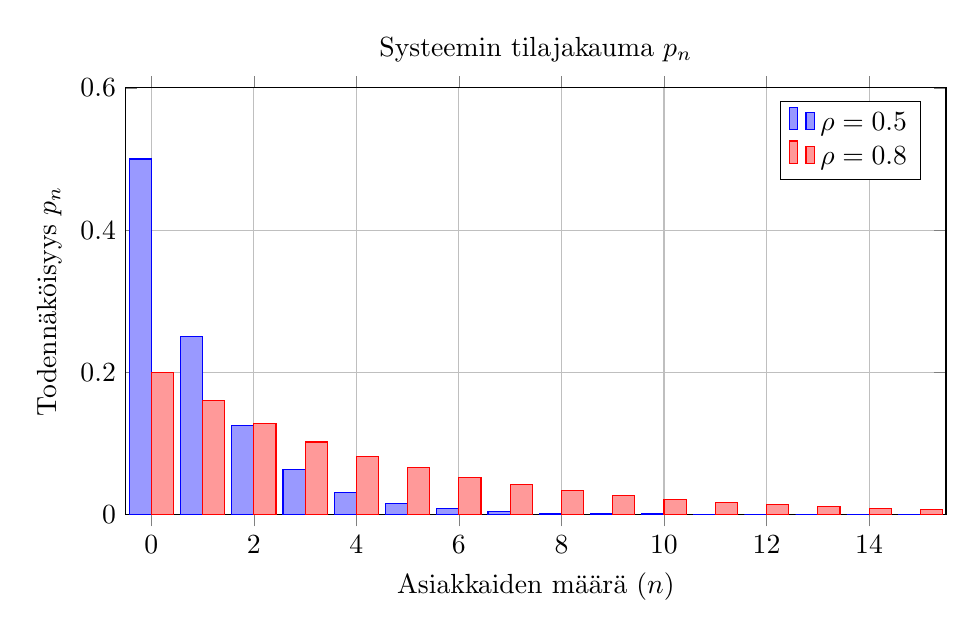
\begin{tikzpicture}
\begin{axis}[
    width=12cm, height=7cm,
    title={Systeemin tilajakauma $p_n$},
    xlabel={Asiakkaiden määrä ($n$)},
    ylabel={Todennäköisyys $p_n$},
    xmin=-0.5, xmax=15.5,
    ymin=0, ymax=0.6,
    ybar=0pt,
    bar width=8pt,
    legend pos=north east,
    grid=major
]
    % Tapaus 1: Rho = 0.5
    \addplot[fill=blue!40, draw=blue] coordinates {
        (0,0.500) (1,0.250) (2,0.125) (3,0.063) (4,0.031)
        (5,0.016) (6,0.008) (7,0.004) (8,0.002) (9,0.001)
        (10,0.001) (11,0.000) (12,0.000) (13,0.000) (14,0.000) (15,0.000)
    };
    \addlegendentry{$\rho = 0.5$}

    % Tapaus 2: Rho = 0.8
    \addplot[fill=red!40, draw=red] coordinates {
        (0,0.200) (1,0.160) (2,0.128) (3,0.102) (4,0.082)
        (5,0.066) (6,0.052) (7,0.042) (8,0.034) (9,0.027)
        (10,0.021) (11,0.017) (12,0.014) (13,0.011) (14,0.009) (15,0.007)
    };
    \addlegendentry{$\rho = 0.8$}
    
\end{axis}
\end{tikzpicture}
\end{center}




\newpage
\subsection{Odotettu asiakasmäärä $L$}

Olkoon satunnaismuuttuja $N$ asiakkaiden lukumäärä systeemissä. Äsken johdettu $p_n$ on muuttujan $N$ todennäköisyysfunktio, eli $P(N=n) = p_n$.
Odotusarvo lasketaan summaamalla jokainen tila painotettuna niiden todennäköisyyksillä:
\begin{equation*}
    L = E[N] = \sum_{n=0}^{\infty} n p_n = (1-\rho) \sum_{n=0}^{\infty} n \rho^n
\end{equation*}

Summan $\sum n \rho^n$ laskemiseksi tarkastellaan tuttua geometrista sarjaa funktiota:
\begin{equation*}
    \sum_{n=0}^{\infty} x^n = \frac{1}{1-x}, \quad |x| < 1
\end{equation*}
Derivoidaan yhtälö puolittain muuttujan $x$ suhteen:
\begin{align*}
    \frac{d}{dx} \sum_{n=0}^{\infty} x^n &= \frac{d}{dx} (1-x)^{-1} \\
    \sum_{n=1}^{\infty} n x^{n-1} &= (-1)(1-x)^{-2}(-1) = \frac{1}{(1-x)^2}
\end{align*}
Kerrotaan puolittain $x$:llä, jolloin saadaan haluttu muoto:
\begin{equation*}
    \sum_{n=1}^{\infty} n x^n = \frac{x}{(1-x)^2}
\end{equation*}

Sijoitetaan tämä tulos (missä $x=\rho$) alkuperäiseen odotusarvon lausekkeeseen:
\begin{align*}
    L &= (1-\rho) \cdot \frac{\rho}{(1-\rho)^2} \\
    L &= \frac{\rho}{1-\rho}
\end{align*}

Palautetaan alkuperäiset muuttujat sijoittamalla $\rho = \frac{\lambda}{x\mu}$:
\begin{equation*}
    L(x) = \frac{\frac{\lambda}{x\mu}}{1 - \frac{\lambda}{x\mu}} = \frac{\lambda}{x\mu - \lambda}
\end{equation*}

Eli odotettu asiakasmäärä on: $\frac{\lambda}{x\mu - \lambda}$


% TÄHÄN TULEE LOPPUTULOS W(x) (Little's Law)

\newpage

\section{Optimointiongelma}

\subsection{Ongelman asettelu}
Minimoitava tavoitefunktio ja rajoitteet:

% TÄHÄN TULEE KAAVAT

\vspace{3cm}

\subsection{Lagrangen menetelmä}

Muodostetaan Lagrangen funktio $\mathcal{L}(x_1, x_2, \alpha)$:

% TÄHÄN TULEE LAGRANGEN FUNKTIO

\vspace{3cm}

Ratkaistaan KKT-ehdot (osittaisderivaatat nollaksi):

% TÄHÄN TULEE DERIVOINTI JA YHTÄLÖRYHMÄN RATKAISU

\vspace{8cm}

\subsection{Lopputulos}

% TÄHÄN TULEE LOPULLISET KAAVAT

\end{document}